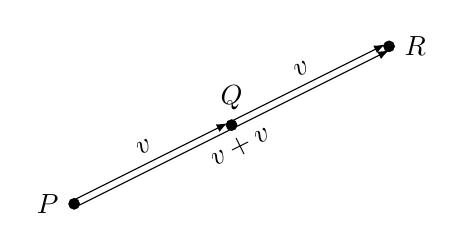
\begin{tikzpicture}[
	point/.style={circle,draw,very thin,fill,inner sep=0pt,minimum size=4pt},
	vector/.style={-latex},
]
	\node[point] at (0,0) (p) [label=left:{$P$}] {};
	\node[point] at (2,1) (q) [label=above:{$Q$}] {};
	\node[point] at (4,2) (r) [label=right:{$R$}] {};
	\draw[vector] (0,0.05) to node[above,sloped] {$\uvec{v}$} (1.95,1.025);
	\draw[vector] (2,1.05) to node[above,sloped] {$\uvec{v}$} (3.95,2.025);
	\draw[vector] (0,-0.05) to node[below,sloped] {$\uvec{v}+\uvec{v}$} (4,1.95);
\end{tikzpicture}
